\chapter{Modern Symmetric-Key Cryptography}
\label{ch:symmetric}

In this section, we transition from classical cryptography, which was largely done by hand, to modern cryptography, an age which is marked by the use of machines and computers. While simple cipher devices, such as the scytale \index{scytale} and cipher disks, were used for many hundreds of years, the first truly mechanical cipher machines \index{cipher machine} were first designed, patented, and built beginning in the late 1910s, around the end of World War I \cite{hac, singh}. Specific independent inventors included the American Edward Hebern, \index{Hebern, Arthur} the Swede Arvid Damm, \index{Damm, Arvid} the Dutchman Alexander Koch, \index{Koch, Alexander} and the German Arthur Scherbius. \index{Scherbius, Arthur} Scherbius is the most famous of this group as the inventor of the Enigma \index{Enigma} machine, used by the Germans in World War II. Use of cipher machines reached its peak during World War II, but various machines were used into the 1970s and 1980s.

It became increasingly painstaking to cryptanalyze these cipher machines by hand, so Allied cryptanalysts, notably the British cryptanalysts Alan Turing \index{Turing, Alan} and Max Newman \index{Newman, Max} invented machines to crack messages that were intercepted from various Axis nations \cite{singh}. Turing first developed the concept of a programmable computer, though in 1823 Babbage \index{Babbage, Charles} was the first to design a machanical calculator. Newman took Turing's ideas and made a blueprint for the first programmable computer, Colossus, \index{Colossus} which was built in 1943. After the war, Colossus and its blueprints were destroyed. However, in 1945, the first (unclassified) programmable computer, ENIAC, was built by J. Presper Eckert and John Mauchly of the University of Pennsylvania \cite {singh}. With the birth of the computer age, all text was internally represented in binary. Since then, virtually all modern symmetric ciphers are described in binary, so aside from Section \ref{sssec:rotor}, we will assume that all plaintexts, keys, and ciphertexts are in binary.

This switch from written text to binary resulted in the codification of various standards for translating text to binary. Some common methods are ASCII \index{ASCII} (American Standard Code for Information Interchange), Extended ASCII, \index{ASCII, Extended}\index{Extended ASCII} and UTF-8, \index{UTF-8} the latter of which is the most common standard in use today. ASCII represents letters and other symbols as a string of 7 bits, one bit shy of a byte, so Extended ASCII uses an eighth bit to represent 128 additional characters. UTF-8 contains ASCII as a subset and allows for the digitization of virtually all international characters and symbols. The following is an extended ASCII table. The labels of the rows and columns represent the hexadecimal digits of the given row or column. So the letter {\tt A} is encoded as the hexadecimal number {\tt 41}, which in binary would be {\tt 01000110}. The boxed entries are various control commands, such as {\tt 20} (SPACE) and {\tt 7F} (DELETE).


\begin{center}
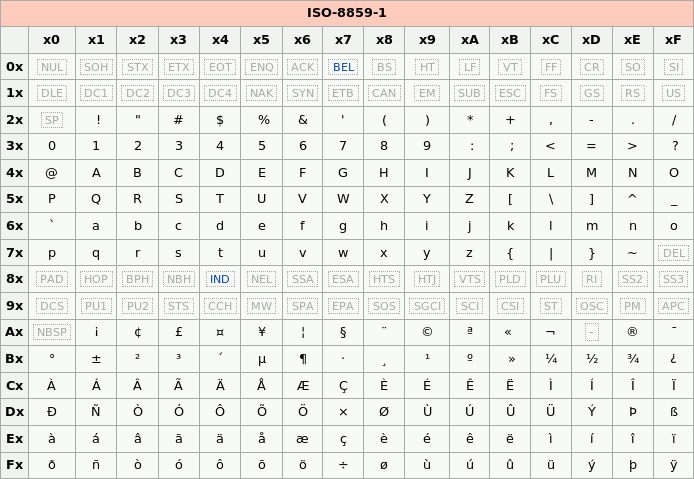
\includegraphics[width=0.9\textwidth]{img/ext-ascii.png}
\end{center}

With this historical and technical background established, we will explore the two main types of modern substitution ciphers: stream ciphers and block ciphers.

	\section{Stream Ciphers}

All of the cryptosystems that we have considered so far fall under the category of {\bf stream ciphers}.  \index{stream cipher} Here is a formal definition.

	\begin{definition}
	A {\bf stream cipher} is a substitution cipher in which the plaintext is encrypted one character (e.g., a letter, bit, or byte) at a time.
	\end{definition}

The following are examples of stream ciphers used since 1900. We won't spend time studying mechanical (e.g. rotor) machines in depth, but are included since they played an important role in cryptographic history.  Stream ciphers are used frequently to encrypt streaming content, such as cell phone calls and internet traffic, because of its speed, simplicity, security, and the flexibility to be used when the length of the plaintext is unknown.

		\subsection{Mechanical Cipher Machines}
		\label{sssec:rotor}

The following are examples of some mechanical cipher machines that were in use from the late 1910s into the 1980s.

		\begin{itemize}
			\item A-21 (Arvid Damm)
			\item Enigma (Arthur Scherbius)
			\item Hebern Machine (Edward Hebern)
			\item KL-51 (NSA)
			\item Lorenz (Germany)
			\item M209-A (Sold to the United States by Boris Hagelin)
			\item PURPLE (97-shiki O-bun in-ji-ki)
		\end{itemize}

	Read \S 2.12 of \cite{tw}

		\subsection{Random and Pseudorandom Number Generators}

So if a one-time pad \index{one-time pad} offers perfect security, an obvious solution would be to somehow generate a random or pseudorandom {\bf keystream}, \index{keystream} a stream of bits to be used as the key, and use a bit-wise addition, modulo $2$, also called a bit-wise {\bf XOR}, \index{XOR} or $\oplus$, to combine it with the plaintext. In this case, the sender and receiver would have to agree on a method to generate a random or pseudorandom sequence of bits and perhaps agree on an additional key (called a {\bf seed}\index{seed}) for the pseudorandom number generator. Before we proceed, it will help to define some terms. (See Chapter 5 of \cite{hac}.)

\begin{definition}
A {\bf random number generator} \index{random number generator} is a device or algorithm which outputs a sequence of statistically independent and unbiased numbers \cite{hac}.
\end{definition}
Typically, the numbers we will generate are binary digits, or bits, so we may alternatively call such a generator a {\bf random bit generator}.

\begin{definition}
A {\bf pseudorandom number generator} \index{pseudorandom number generator} (PRNG) is a deterministic algorithm which inputs a truly random digit sequence and outputs an expanded digit sequence which ``appears" to be random. The input to the PRNG is called the {\bf seed}, \index{seed} while the output of the PRNG is called a {\bf pseudorandom digit sequence} \cite{hac}.
\end{definition}
Again, we will typically be generating a sequence of pseudorandom bits.

The one word in the definition of a PRNG that needs further elaboration in order for this definition to be rigorous is the word {\em appear}. What does it mean to {\em appear} random? There are various statistical tests to measure randomness. (See \S5.4.4 of \cite{hac} or the Statistical Test Suite developed by NIST \cite{nist}.) If a sequence of numbers passes all the tests for randomness in a given test suite, then we say the the sequence {\bf appears} random.

Now just because a number sequence is pseudorandom, doesn't mean that it's secure enough for cryptographic purposes. To this end, we introduce another term.

\begin{definition}
A PRNG is {\bf cryptographically secure} \index{cryptographically secure} if
	\begin{enumerate}
		\item its seed \index{seed} is sufficiently long to make it infeasible to perform a brute-force attack on the PRNG by testing all possible seeds and
		\item given any sequence of digits generated by the PRNG, there is no polynomial-time algorithm that can predict the next digit with any degree of certainty (e.g., with probability greater than $1/2$ for a pseudorandom bit string).
	\end{enumerate}
We may soften this definition somewhat by allowing the sequence of digits in point \#2 to be sufficiently short, specifically, shorter than the length of any intended plaintext or short enough to be stored digitally. It is also common to weaken point \#2 to say that predicting the next bit or digit must be at least as hard as a brute-force attack. We may also add in an assumption that there is sufficient security because the PRNG is based on a mathematical problem that is believed to be solvable in polynomial time.
\end{definition}

Read \S 2.10 of \cite{tw}.


As a note on chronology, the {\bf Blum-Blum-Shub} PRNG \index{Blum-Blum-Shub} (BBS) was published in 1986 and it was motivated by developments in public-key cryptography, notably the RSA \index{RSA} cryptosystem, which we will discuss in Section \ref{ch:pkc}. Its claim of cryptographic security is based on the belief that the {\bf quadratic residuosity problem}\index{quadratic residuosity problem} is computationally difficult when the modulus $n$ is a large composite number. In other words, given $n=pq$, it is believed to be hard to determine if for some $a\in\Z_n$, whether the congruence $x^2 \equiv a \ppmod{n}$ has a solution. This problem is easy if the modulus is prime, so this PRNG relies on the belief that the {\bf integer factorization problem}\index{integer factorization problem} is difficult for large composite integers.


\begin{problem}
\label{prob:lincong1}  [10 points]
Let $x_n = 7 x_{n-1} + 1 \ppmod{10}$ be a linear congruential generator. \index{linear congruential generator} What are all the possible period lengths of this recurrence?
\end{problem}

\begin{problem}
\label{prob:lincong2}  [10 points]
Let $x_n = 7 x_{n-1} + 1 \ppmod{11}$ be a linear congruential generator. \index{linear congruential generator} What are all the possible period lengths of this recurrence?
\end{problem}

\begin{problem}
\label{prob:lincong3}  [10 points]
Based on the results of Problems \ref{prob:lincong1} and \ref{prob:lincong2}, make a conjecture about how the modulus relates to the possible period lengths of a linear congruential generator.\index{linear congruential generator} (You may want to experiment further.)
\end{problem}

\begin{problem}
\label{prob:lincong4}  [10 points]
Suppose that you intercepted a message that used the output of a linear congruential generator \index{linear congruential generator} as the key. Suppose that you determined that the modulus is $17$ and that the first three elements of the keystream were 7, 13, and 9. Based on this information, determine the linear congruential generator that was used and the next three elements of the keystream.
\end{problem}

\begin{problem}
\label{prob:lincong5} [15 points] Suppose that you intercepted a message that used the output of a linear congruential generator \index{linear congruential generator} as the key. Suppose that you determined that the modulus is $997$ and that the first three elements of the keystream were 6, 795, and 978. Based on this information, determine the linear congruential generator that was used and the next three elements of the keystream.
\end{problem}

\begin{problem}
\label{prob:lincong6}  [20 points]
Suppose that you intercepted a message that used the output of a linear congruential generator \index{linear congruential generator} as the key and determined the first ten elements of the keystream: 51, 93, 68, 39, 17, 7, 73, 6, 2, and 9. Based on this information, determine the linear congruential generator that was used and the next three elements of the keystream.
\end{problem}

\begin{problem}  [10 points]
Let $p = 263$ and $q = 283$. If we wanted to use these primes to use BBS as a cryptographically secure PRNG, how many bits could we use with each iteration so generate a cryptographically secure pseudorandom bit stream? Use any seed of your choice to generate 12 pseudorandom bits.
\end{problem}

\begin{problem}
\label{prob:bbs2}  [10 points]
If you wanted to use the Blum-Blum-Shub PRNG as a cryptographically secure PRNG and wanted to use 4 bits with each iteration, how many bits would the modulus $n$ have to have? How many bits would $p$ and $q$ have to have?
\end{problem}

\begin{problem}
\label{prob:bbs3}  [15 points]
As a follow-up to Problem \ref{prob:bbs2}, find primes $p$ and $q$ that would allow you to extract four pseudorandom bits with each iteration. Use the resulting BBS PRNG to generate 32 pseudorandom bits (8 bytes) and encrypt ``{\tt MAT 337!}" using extended-ASCII to encode the eight characters.
\end{problem}

\begin{problem}
\label{prob:bbs4}  [10 points]
Let $p=7$ and $q=11$. What are the possible period lengths of the BBS PRNG?
\end{problem}

\begin{problem}
\label{prob:bbs5}  [10 points]
If $n=pq$ is the modulus of a BBS PRNG, what are some seeds that you would obviously want to avoid?
\end{problem}

\begin{problem}
\label{prob:bbs6} [15 points]
If $n = pq$, and $x_{k+1} = x_k^2\ppmod{n}$, then
$$x_k = \left(x_0^{2^k\ppmod{\lambda(n)}}\right)\ppmod{n} \enspace ,$$
where $\lambda(n) = \lcm((p-1)(q-1))$.
\end{problem}

		\subsection{Other Cryptographically Secure PRNGs}

	The following is a list of other PRNGs that are considered to be cryptographically secure.

		\begin{itemize}
			\item ANSI X9.17 Standard
			\item Blum-Micali
			\item CryptGenRandom
			\item Fortuna
			\item ISAAC
			\item NIST SP 800-90A Standards
			\item Yarrow
		\end{itemize}

\begin{problem} [15 points]
	Do some basic research on one of the PRNGs in the list above. Describe the method, state where and/or how the PRNG is used in practice, and make some brief comments on its security. If it is feasible, generate a cryptographically secure pseudorandom bit sequence by hand or write a program to generate such a sequence.
\end{problem}

		\subsection{Linear Feedback Shift Registers}

		Read \S 2.11 of \cite{tw}.

\begin{problem} [10 points]
\S 2.13 Exercise \#19
\end{problem}

\begin{problem} [10 points]
\S 2.13 Exercise \#20
\end{problem}

\begin{problem} [10 points]
\S 2.13 Exercise \#21
\end{problem}

\begin{problem} [10 points]
\S 2.13 Exercise \#22
\end{problem}

\begin{problem} [15 points]
\S 2.14 Computer Problem \#11
\end{problem}

\begin{problem} [15 points]
\S 2.14 Computer Problem \#12
\end{problem}

\begin{problem} [15 points]
\S 2.14 Computer Problem \#13
\end{problem}

		\subsection{Examples of Modern Stream Ciphers}

	\begin{itemize}
		\item A5/1
		\item ChaCha (Dan Bernstein)
		\item ISAAC (Robert Jenkins, Jr.)
		\item RC4 (Ron Rivest)
		\item Salsa20 (Dan Bernstein)
		\item SEAL (Phillip Rogaway and Don Coppersmith)
		\item Speck (NSA)
		\item Spritz (Ron Rivest)
	\end{itemize}

\begin{problem} [15 points]
	Explore one of the stream ciphers listed above, or any other stream cipher. Include:
	\begin{enumerate}
		\item A mathematical description of the cipher, with pictures if it helps to elucidate the description.
		\item Encrypt your initials using the equivalent non-extended ASCII encoding with the stream cipher and a key of your choice. %(This can be done by hand or by implementing this on a computer.)
		\item Give some examples of applications that use the stream cipher in practice.
		\item Briefly describe the security of the stream cipher. Are there any attacks on the stream cipher that are better than a brute-force attack of the key? If so, are these attacks on the cipher practical or impractical? (This is not intended to be overly technical and should be understood by anyone else in the class.)
	\end{enumerate}
\end{problem}

The disadvantage of just using a stream cipher to encrypt information is that the ciphertext is prone to a {\bf bit-flipping attack}, \index{bit flipping attack}, a form of a man-in-the-middle attack, \index{man-in-the-middle attack} in which an eavesdropper intercepts the message and changes some of the ciphertext. For example, if Eve, the eavesdropper intercepted a message from Alice to Bob that read ``Alice is sending Bob 4 Bitcoins" and she knew the structure of the message, then she could XOR the binary equivalent of ``Bob $\xor$ Eve" in the appropriate location of the message thus changing it to ``Alice is sending Eve 4 Bitcoins" and Eve is suddenly 4 Bitcoins richer! To avoid such an attack, ciphertexts that were encrypted with a stream cipher should include some kind of authentication, such as a message authentication code (MAC) \index{message authentication code}, so that any tampering of the ciphertext would be detected. Man-in-the-middle attacks will be discussed more completely in Section \ref{sssec:mitm} and MACs will be discussed in Section \ref{sssec:mac}.

	\section{Block Ciphers}

In contrast to a stream cipher, {\bf block ciphers} \index{block cipher} encrypt multiple characters, bits, or bytes, called {\bf blocks}, \index{block} at a time. Some classical cryptosystems encrypted blocks of two letters at a time, such as the Playfair Cipher, while modern block ciphers will encrypt plaintext in blocks of 64 or 128 bits, for example. We include two classical cryptosystems here as motivation for modern block ciphers, so with the classical ciphers, the Playfair cipher (\S \ref{sssec:playfair}) and the Hill cipher (\S \ref{sssec:hill}), plaintext and ciphertext will use elements of $\LL$, while subsequent sections will use binary.

		\subsection{The Playfair Cipher} \index{Playfair cipher}
		\label{sssec:playfair}
		Read \S 2.6 of \cite{tw}.

\begin{problem}
\label{prob:playfair}  [10 points]
Encrypt a plaintext of your choice with at least 100 characters with the Playfair cipher using a key your choice. The rest of the class will be challenged later to cryptanalyze the ciphertext.
\end{problem}
\begin{problem}  [15 points]
Recover the plaintext from a peer's ciphertext, which was encrypted using the Playfair cipher in Probem \ref{prob:playfair}.
\end{problem}

		\subsection{The Hill Cipher} \index{Hill cipher}
		\label{sssec:hill}
		Read \S 2.7 of \cite{tw}.

As noted in \cite{tw}, the Hill cipher was not often used, but is notable for being the first to utilize algebraic techniques. The cipher uses distinct encryption and decryption functions (namely, linear transformations) which are inverses of each other. Its downside is that the decryption function is easy to determine from the encryption function because finding the inverse of an invertible matrix is computationally easy.

\begin{problem} [10 points]
\S 2.13 Exercise \#13
\end{problem}

\begin{problem} [10 points]
\S 2.13 Exercise \#14
\end{problem}

\begin{problem} [15 points]
\S 2.13 Exercise \#15
\end{problem}

\begin{problem} [15 points]
\S 2.13 Exercise \#16
\end{problem}

\begin{problem} [15 points]
\S 2.13 Exercise \#17
\end{problem}

\begin{problem} [20 points]
\S 2.13 Exercise \#18
\end{problem}

\begin{problem} [10 points]
\S 2.14 Computer Problem \#10
\end{problem}

\begin{problem}
\label{prob:hill1}  [10 points]
Give an example of an invertible $3\times 3$ matrix with entries in $\Z_{26}$ and find the inverse of the matrix.
\end{problem}

\begin{problem}  [10 points]
How many invertible $2\times 2$ matrices with entries in $\Z_{26}$ are there?
\end{problem}

\begin{problem}  [10 points]
How many invertible $2\times 2$ matrices with entries in $\Z_{37}$ are there?
\end{problem}

\begin{problem}  [10 points]
How many invertible $3\times 3$ matrices with entries in $\Z_{26}$ are there?
\end{problem}

\begin{problem}  [10 points]
How many invertible $3\times 3$ matrices with entries in $\Z_{37}$ are there?
\end{problem}

\begin{problem}  [15 points]
Let $n\in\N$ and let $p$ be a prime. How many invertible $n\times n$ matrices with entries in $\Z_p$ are there?
\end{problem}

\begin{problem}
\label{prob:hill2}  [10 points]
Encrypt a plaintext of your choice with at least 100 characters with the Hill cipher using a key your choice. (This key could be any matrix found in Problem \ref{prob:hill1}. The rest of the class will be challenged later to cryptanalyze the ciphertext.
\end{problem}
\begin{problem}  [10 points if the key is known; 20 points if the key is unknown]
Recover the plaintext from a peer's ciphertext, which was encrypted using the Hill cipher in Problem \ref{prob:hill2}.
\end{problem}


		\subsection{Data Encryption Standard (DES)} \index{DES}\index{Data Encryption Standard}\index{Lucifer}

		Read \S 4.1, 2, 4, and 5 of \cite{tw}.

\paragraph*{Discussion} What are some of the big ideas in the development of DES? What is a Feistel system?

\begin{definition}
	A function $f$ is called a {\bf pseudorandom function} \index{pseudorandom function} if $f$ is an efficient deterministic function whose output cannot be efficiently distinguished from random data.
\end{definition}

\paragraph*{Discussion} Explain why the designers of DES needed a function $f$, as denoted in the description of DES and a simplified DES-type algorithm, that is a pseudorandom function.

\begin{center}
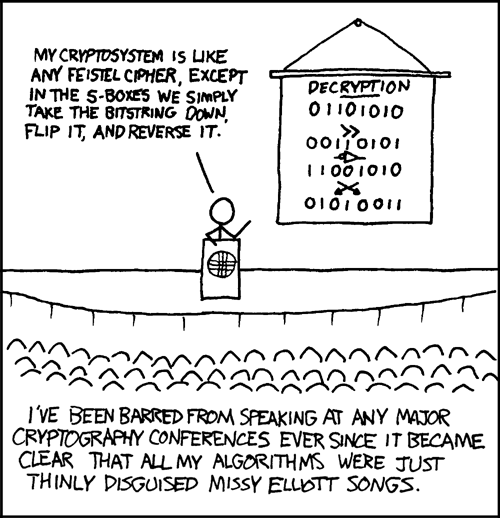
\includegraphics[width=0.5\textwidth]{img/cryptography-xkcd.png}
\end{center}

\begin{problem} [20 points]
Briefly describe the Electronic Codebook (ECB), Cipher Block Chaining (CBC), Cipher Feedback (CFB),  Output Feedback (OFB), and Counter (CTR) modes of operation for block ciphers. What are any strengths and/or weaknesses of each?
\end{problem}
		\subsection{Other Feistel-based Block Ciphers}

		\begin{itemize}
			\item Blowfish
			\item Camellia
			\item CAST-128 and CAST-256
			\item RC5
			\item RC6
			\item Skipjack
			\item TEA (Tiny Encryption Algorithm) and variants
			\item Twofish
			\item 3DES (Triple DES) (\S 4.6 of \cite{tw})
		\end{itemize}

\begin{problem}  [20 points]
Although many block ciphers are proprietary, the description of many block ciphers have been published. Do some basic research on one of the Feistel-based block ciphers above. Answer as many of the following questions as you can.
	\begin{enumerate}
		\item Who created the cipher, what is (are) their affiliation(s), and when was it developed?
		\item What applications use the block cipher?
		\item What size keys does the cipher use and what is the block size that the cipher uses?
		\item Does the cipher make any modifications to the pure Feistel structure?
		\item Describe the pseudorandom function $f$ and any design considerations of the creators.
		\item Briefly state the best known attacks on the cipher. (You will likely come across terminology that we haven't defined yet. That's OK, much of it is quite technical, and later we'll only get a very rough idea of some of the concepts. You're certainly not expected to understand how differential cryptanalysis works, for example.)
	\end{enumerate}
\end{problem}

		\subsection{Other Block Cipher Designs and Components}

		\begin{itemize}
			\item Key Schedule
			\item S-box (substitution box)
			\item P-box (permutation box)
			\item Lai-Massey Scheme
			\begin{itemize}
				\item IDEA
			\end{itemize}
		\end{itemize}

		\subsection{Advanced Encryption Standard (AES)}\index{AES}\index{Advanced Encryption Standard}\index{Rijndael}

		Read Chapter 5 of \cite{tw}.



	\section{Cryptanalysis of Stream and Block Ciphers}

		\subsection{Brute Force Attack}

                \begin{definition}
                  A {\bf brute force attack}\index{brute force attack} on a cryptogram is a cryptanalytic technique in which keys are systematically used to decrypt until the correct key is found.
                \end{definition}

                \begin{problem} [10 points]
                  If a message is encrypted using a 64-bit key, what is an upper bound on the amount of time it would take 1000 computers to crack the ciphertext if each computer can test a million keys per second?
                \end{problem}

                \begin{problem} [10 points]
                  If a message is encrypted using a 128-bit key, what is an upper bound on the amount of time it would take a billion computers to crack the ciphertext if each computer can test a billion keys per second?
                \end{problem}

		\subsection{Known-Plaintext Attacks}

		Read \S 1.1.1 \#2 of \cite{tw}.

		\subsection{Chosen-Plaintext Attacks}

		Read \S 1.1.1 \#3 of \cite{tw}.

		\subsection{Differential Cryptanalysis}

		Read \S 4.3  of \cite{tw}.

		\subsection{Meet-in-the-Middle Attacks}
		\label{sssec:mitm}

		Read \S 4.7 of \cite{tw}.

		\subsection{Black-bag cryptanalysis}

			This isn't mathematical cryptanalysis, but {\bf black-bag cryptanalysis} \index{black-bag cryptanalysis} refers to a generally more practical form of cryptanalysis in which encryption and/or decryption keys or passwords are stolen by any number of means. This may include the following.
		\begin{itemize}
			\item Installation of Trojan horse software on a computer to send passwords to an attacker.
			\item Installation of a keystroke logger to record typing.
			\item Finding a password written on a piece of paper.
			\item Installation of bugs (video and/or audio surveillance) in a room.
			\item Reading electromagnetic transmissions from an electronic device.
			\item Social engineering
		\end{itemize}
		Despite the nontechnical aspects of black-bag methods, it is important to be aware of these forms of cryptanalysis since otherwise unbreakable encryption can be broken if the key is revealed on account of carelessness.

		\subsection{Rubber-hose cryptanalysis}

\begin{center}
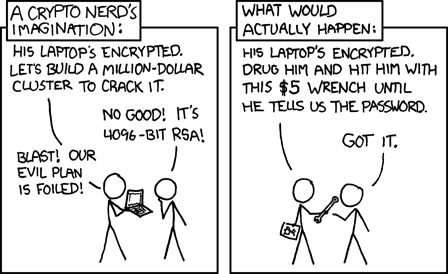
\includegraphics{img/security-xkcd.png}
\end{center}

			As with black-bag methods, {\bf rubber-hose cryptanalysis} \index{rubber-hose cryptanalysis} is not a mathematical technique, but rather any method of recovering encrypted content, a password, or encryption/decryption keys via blackmail, coercion, threats, or torture.


\begin{problem} [15 points]
\S 4.9 Exercise \#1.a.
\end{problem}

\begin{problem} [15 points]
\S 4.9 Exercise \#1.b.
\end{problem}

\begin{problem} [15 points]
\S 4.9 Exercise \#1.c.
\end{problem}

\begin{problem} [10 points]
\S 4.9 Exercise \#2.
\end{problem}

\begin{problem} [15 points]
\S 4.9 Exercise \#3.
\end{problem}

\begin{problem} [15 points]
\S 4.9 Exercise \#4.
\end{problem}

\begin{problem} [15 points]
\S 4.9 Exercise \#5.
\end{problem}

\begin{problem} [15 points]
\S 4.9 Exercise \#6.
\end{problem}

\begin{problem} [15 points]
\S 4.9 Exercise \#7.
\end{problem}

\begin{problem} [10 points]
\S 4.9 Exercise \#8.
\end{problem}

\begin{problem} [15 points]
\S 4.9 Exercise \#9.
\end{problem}

\begin{problem} [10 points]
\S 4.9 Exercise \#10.
\end{problem}

\begin{problem} [10 points]
\S 4.9 Exercise \#11.
\end{problem}

\begin{problem} [15 points]
\S 4.10 Computer Problem \#1.a and 1.b.
\end{problem}

\begin{problem} [10 points]
\S 4.10 Computer Problem \#1.c.
\end{problem}

\begin{problem} [10 points]
\S 4.10 Computer Problem \#1.d.
\end{problem}

\begin{problem} [10 points]
\S 4.10 Computer Problem \#2.
\end{problem}

\begin{problem} [10 points]
Explore a topic that came out of a class discussion or solve a problem inspired by the content of this chapter.
\end{problem}
